\section{Results}

\begin{table}[ht]
  \centering
  \begin{tabular}{|c|c|c|c|c|}
    \hline
    Region & Remote & Local & Potential & Total \\
    \hline
    West Coast & 420 & 90 & 190 & 510 - 610 \\
    Hawaii & 290 & 10 & 90 & 300 - 380 \\
    East Coast & 110 & 170 & 210 & 280 - 320 \\
    Gulf of Mexico & 13 & 50 & 60 & 63-73 \\
    Alaska & 1040 & 960 & 1390 & 2000 - 2430 \\
    Puerto Rico & 6 & 11 & 26 & 17 - 32 \\
    \hline \hline
U.S. TOTAL & 1879 & 1291 & 1966 & 3170 - 3845 \\
\hline
  \end{tabular}
  \caption{Wave resource assessment results by region and totaled for the entire U.S. (all values in TWh/yr). The range in the total column indicates the sum of Remote+Local (lower value) and Remote+Potential (higher value). \note{We need to confirm these values again.}}
  \label{table:totals}
\end{table}


\begin{table}[ht]
  \centering
  \begin{tabular}{|c|c|c|c|}
    \hline
    Region 
    &
      \begin{tabular}{c}
        EPRI 2011 \\ {\it Remote Only} \\ $\mathrm{[TWh/yr]}$
      \end{tabular}
    &
      \begin{tabular}{c}
        New Total \\ TWh/yr
      \end{tabular}
    & \% Change \\
    \hline
    West Coast & 590 & 510 - 610 & -5 $\pm$10 \\
    Hawaii & 130 & 300 - 380 & +160 $\pm$30 \\
    East Coast & 240 & 280 - 320 & 25 $\pm$8 \\
    Gulf of Mexico & 80 & 63 - 73 & -15 $\pm$7 \\
    Alaska & 1570 & 2000 - 2430 & +40 $\pm$15 \\
    Puerto Rico & 30 & 17 - 32 & -20 $\pm$25 \\
    \hline \hline
    U.S. TOTAL  & 2640 & 3170 - 3845 & +33 $\pm$ 13 \\
    \hline
  \end{tabular}
  \caption{Wave resource totals compared to 2011 results (all values in TWh/yr).}
  \label{tab:total-compare}
\end{table}

\begin{figure}[ht]
  \centering
  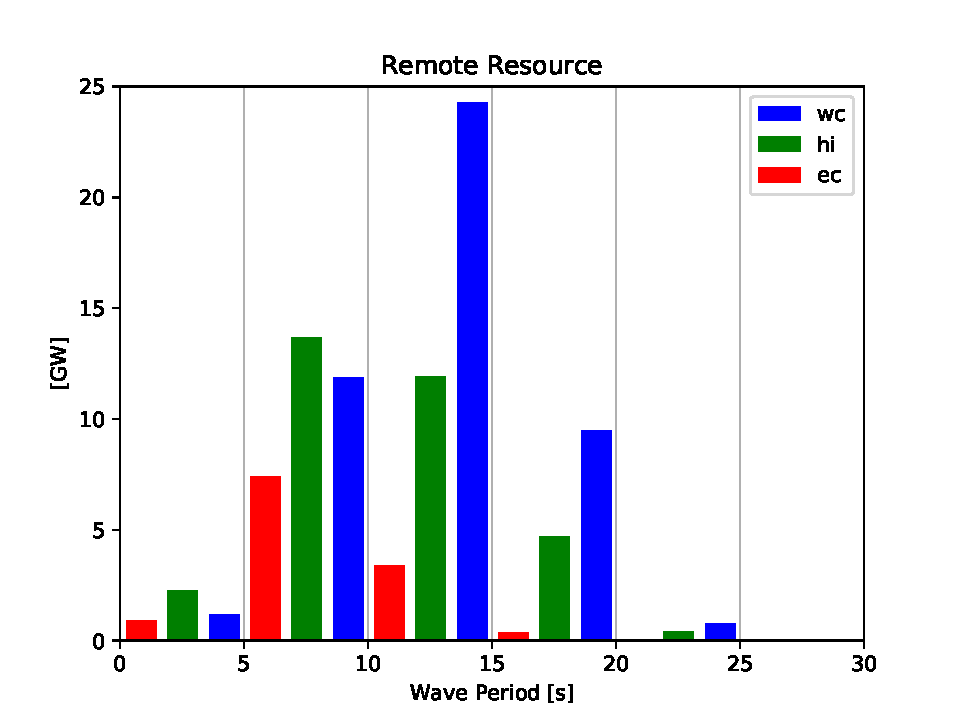
\includegraphics[width=\linewidth]{../fig/RemoteResource_Freq01.pdf}
  \caption{Remote resource contained in each wave period band (0-5 seconds, 5-10 seconds, etc.) for the west coast (wc), Hawaii (hi), and the east coast (ec).}
  \label{fig:remote-freq}
\end{figure}

\begin{figure}[ht]
  \centering
  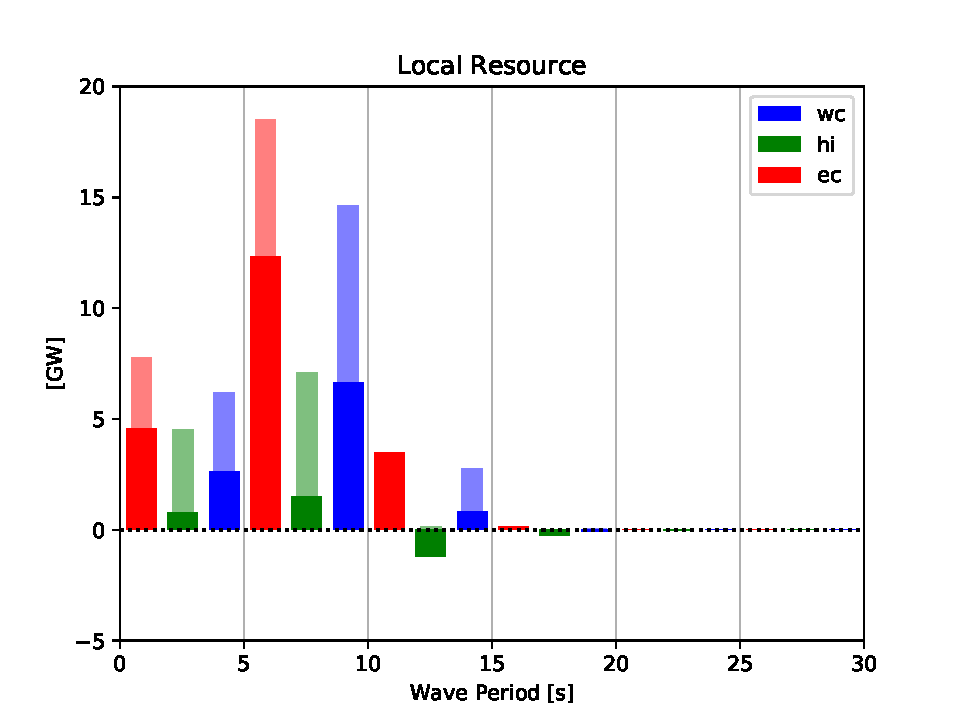
\includegraphics[width=\linewidth]{../fig/LocalResource_Freq01.pdf}
  \caption{Local (thick solid bars) and potential (narrow pale bars) resource contained in each wave period band (0-5 seconds, 5-10 seconds, etc.) for the west coast (wc), Hawaii (hi), and the east coast (ec).}
  \label{fig:remote-freq}
\end{figure}

\begin{itemize}
\item National total plus Regional/State-by-state breakdown of resource.
\item Plots of ‘remote’ resource vs. distance from shore (Figure 5). ... How does this compare with local resource vs. distance from shore?
\item Remote resource vs. depth. Local resource vs. depth.
\end{itemize}
